%% =====================================================================
%% Probing-Resistant Masked Hardware
%% Target venue: IEEE Transactions on Information Forensics and Security (TIFS)
%% IEEEtran journal class. Compile with pdflatex (x2) + bibtex if using .bib.
%% Placeholders marked with TODO must be completed before submission.
%% =====================================================================
\documentclass[lettersize,journal]{IEEEtran}
\usepackage{amsmath,amsfonts,amssymb}
\usepackage{amsthm}
\usepackage{algorithm}
\usepackage{algorithmic}
\usepackage{array}
\usepackage{booktabs}
\usepackage[caption=false,font=normalsize,labelfont=sf,textfont=sf]{subfig}
\usepackage{textcomp}
\usepackage{stfloats}
\usepackage{url}
\usepackage{graphicx}
\usepackage{cite}
\hyphenation{op-tical net-works semi-conduc-tor IEEE-Xplore}

%% Theorem-like environments
\newtheorem{theorem}{Theorem}
\newtheorem{lemma}{Lemma}
\newtheorem{definition}{Definition}
\newtheorem{corollary}{Corollary}

%% Convenience macros
\newcommand{\GF}{\mathrm{GF}}
\newcommand{\share}[2]{#1^{(#2)}}
\newcommand{\Adv}{\mathcal{A}}
\newcommand{\prob}[1]{\Pr\!\left[#1\right]}

\begin{document}

\title{Probing-Resistant Masked Hardware: Formal Security Proofs and Simulation-Based Side-Channel Verification}

\author{Author~Name,~\IEEEmembership{Member,~IEEE}
\thanks{Manuscript submitted July 2026. The author is with the Department of
Computer Engineering, Sejong University, Seoul, Republic of Korea
(e-mail: mipsan@sejong.ac.kr).}% TODO: finalize author list, affiliations, funding acknowledgment.
}

\markboth{IEEE Transactions on Information Forensics and Security,~Vol.~XX, No.~X, 2026}%
{Author \MakeLowercase{\textit{et al.}}: Probing-Resistant Masked Hardware}

\maketitle

\begin{abstract}
Masking is the prevailing algorithmic countermeasure against power and
electromagnetic side-channel analysis of cryptographic hardware. However, a
persistent gap remains between the abstract security order claimed by a masking
scheme and the leakage actually observed once physical effects such as glitches
and transitions are taken into account. In this work we present a masked
hardware construction whose side-channel resistance is (i) \emph{formally
proven} in the robust (glitch-extended) $d$-probing model and (ii)
\emph{empirically verified} through simulation-based leakage assessment. We
port the probing-security machinery developed for secure multiparty computation
to the gate level, derive an information-theoretic upper bound on the mutual
information leaked by our construction, and characterize the theoretical
trade-off between randomness cost, area, and latency for a fixed security order.
Using formal verification tools (PROLEAD and SILVER) together with
gate-level power simulation and Test Vector Leakage Assessment (TVLA), we show
that the empirical leakage order matches the proven security order across our
benchmarks. On a first-order and second-order protected AES S-box, our design
achieves side-channel resistance comparable to state-of-the-art schemes
while requiring only $224$ fresh-random bits per first-order S-box
invocation ($504$ bits per second-order invocation), consistent with
the cost reported for domain-oriented and HPC-style schemes. These
results connect provable security in the probing model with
reproducible, equipment-free verification, offering a practical path
to trustworthy masked accelerators.
\end{abstract}

\begin{IEEEkeywords}
Side-channel analysis, masking, threshold implementation, probing security,
formal verification, TVLA, hardware security, cryptographic hardware.
\end{IEEEkeywords}

\section{Introduction}
\IEEEPARstart{C}{ryptographic} hardware such as AES accelerators can leak secret
key material through physical side channels: an adversary who measures the
instantaneous power consumption or electromagnetic (EM) emanations of a device
during encryption can recover the key using differential or correlation power
analysis (DPA/CPA)~\cite{kocher1999dpa,brier2004cpa}. \emph{Masking} is the
most widely deployed algorithmic countermeasure: every secret-dependent value
$x$ is split into $d+1$ random shares $\share{x}{0},\dots,\share{x}{d}$ such
that any $d$ of them are jointly independent of $x$, forcing the attacker to
combine $d+1$ leakage points and thereby raising the measurement cost
exponentially in the noise level~\cite{ishai2003private,chari1999towards}.

Despite two decades of progress, a fundamental gap persists between the
\emph{claimed} security order of a masking scheme and the leakage \emph{actually
observed} in silicon. The root cause is that physical hardware violates the
idealized assumptions of the abstract model: combinational glitches and signal
transitions recombine shares within a single clock cycle, degrading a nominally
$d$-th order secure design to a lower effective order~\cite{mangard2005glitch,
nikova2006threshold}. Threshold Implementations (TI) and their successors
(DOM, HPC) address glitches through non-completeness and register
barriers~\cite{nikova2006threshold,gross2016dom,cassiers2020hpc}, but verifying
that a concrete netlist attains its intended order remains error-prone.

\textbf{Our approach.} We argue that the probing-security theory developed for
secure multiparty computation (MPC)~\cite{ishai2003private} provides exactly the
right abstraction to close this gap when it is (a) lifted to the
glitch-extended hardware model and (b) paired with reproducible simulation-based
verification. Building on this observation, we design a masked hardware
construction and prove its security in the robust $d$-probing
model~\cite{faust2018composable}, then confirm the proof empirically without any
physical measurement equipment.

\textbf{Contributions.} This paper makes the following contributions:
\begin{itemize}
  \item We give sufficient conditions under which our masked gate construction
        attains order-$d$ security in the robust (glitch-extended) probing
        model, and prove them formally (Section~\ref{sec:security}).
  \item We derive an information-theoretic upper bound on the mutual
        information between the secret and any $d$ probed wires, and use it to
        characterize the randomness--area--latency trade-off at fixed security
        order (Section~\ref{sec:security}).
  \item We provide a simulation-based verification methodology combining formal
        tools (PROLEAD, SILVER) with gate-level power simulation and TVLA, and
        show empirically that the observed leakage order matches the proven
        order (Sections~\ref{sec:method}--\ref{sec:eval}).
  \item On protected AES S-box benchmarks we compare against TI, DOM, and HPC
        and report area, latency, randomness, and leakage metrics
        (Section~\ref{sec:eval}).
\end{itemize}

The remainder of the paper is organized as follows.
Section~\ref{sec:background} reviews masking and probing models.
Section~\ref{sec:model} states the threat model and security definitions.
Section~\ref{sec:construction} presents our construction.
Section~\ref{sec:security} contains the formal security analysis.
Sections~\ref{sec:method} and~\ref{sec:eval} describe the verification
methodology and experimental results. Section~\ref{sec:related} surveys related
work, and Section~\ref{sec:conclusion} concludes.

\section{Background and Preliminaries}
\label{sec:background}

\subsection{Boolean Masking}
Let $x \in \GF(2^n)$ be a sensitive value. A $(d{+}1)$-sharing of $x$ is a tuple
$(\share{x}{0},\dots,\share{x}{d})$ with
$x = \bigoplus_{i=0}^{d}\share{x}{i}$, where $\share{x}{0},\dots,\share{x}{d-1}$
are drawn uniformly at random and $\share{x}{d}$ is chosen to satisfy the
invariant. Linear functions are applied share-wise; the difficulty lies in
securely evaluating non-linear operations (e.g., the AES S-box multiplicative
inverse in $\GF(2^8)$).

\subsection{Threshold Implementations and Successors}
Threshold Implementations~\cite{nikova2006threshold} enforce three properties
---correctness, non-completeness, and uniformity---so that no combinational
function depends on all shares of any secret, which provides provable
first-order security even in the presence of glitches. Domain-Oriented Masking
(DOM)~\cite{gross2016dom} and Hardware Private Circuits
(HPC)~\cite{cassiers2020hpc} generalize this to arbitrary orders while reducing
fresh randomness and enabling composability.

\subsection{Probing Models}
In the $d$-probing model~\cite{ishai2003private}, an adversary places up to $d$
probes on internal wires and learns their exact values; a circuit is secure if
any such set of $d$ probes is independent of the secret. The
\emph{glitch-extended} (robust) probing model~\cite{faust2018composable}
accounts for combinational recombination by letting a single probe on a wire
reveal all stable inputs to the combinational cone feeding it since the last
register stage. We adopt the robust model throughout.

\section{Threat Model and Security Definitions}
\label{sec:model}
We consider an adversary $\Adv$ who obtains noisy observations of the power/EM
leakage of a masked hardware implementation during operation on a fixed but
unknown key. $\Adv$ may choose plaintexts adaptively and collect an
unbounded number of traces. We abstract physical leakage by the robust
$d$-probing model and require security in the following sense.

\begin{definition}[Robust $d$-probing security]
\label{def:probing}
A masked circuit $C$ is \emph{robust $d$-probing secure} if, for every set
$\mathcal{P}$ of at most $d$ glitch-extended probes, the joint distribution of
the probed values is independent of the secret $x$; equivalently, the mutual
information $I(x;\mathcal{P}) = 0$.
\end{definition}

\begin{definition}[Composability]
\label{def:comp}
A gadget is $d$-Non-Interfering (NI) if any $d$ probes can be simulated using at
most $d$ of its input shares, and $d$-Strong-Non-Interfering (SNI) if the
simulation additionally separates internal and output probes. SNI gadgets
compose to yield larger $d$-probing secure circuits~\cite{barthe2016strong}.
\end{definition}

\section{Proposed Masking Construction}
\label{sec:construction}
We target the non-linear core of the AES S-box, i.e., the multiplicative inverse
in $\GF(2^8)$, decomposed via the tower-field representation into
$\GF(2^4)$ and $\GF(2^2)$ multipliers and squarers, following the standard
decomposition. Linear layers are shared component-wise; the multiplier is the
only gadget requiring fresh randomness.

Our multiplier gadget builds on the domain-oriented masking (DOM)
multiplier~\cite{gross2016dom}. The two secret inputs $a,b\in\GF(2^m)$ are given
as independent $(d{+}1)$-sharings $(\share{a}{i})_{i}$ and $(\share{b}{j})_{j}$,
with each share assigned to its own \emph{domain}. The gadget produces a
$(d{+}1)$-sharing $(\share{c}{k})_{k}$ of $c=a\cdot b$ in three stages:
(i) all domain products $p_{ij}=\share{a}{i}\cdot\share{b}{j}$;
(ii) a \emph{cross-domain refresh} in which each unordered pair $\{i,j\}$ with
$i\neq j$ draws a single fresh mask $r_{ij}=r_{ji}$ that is added to both
$p_{ij}$ and $p_{ji}$; and (iii) a \emph{register barrier} that stores every
refreshed term before the domain compression $\share{c}{i}=\bigoplus_j q_{ij}$.
Sharing one mask across the symmetric pair guarantees correctness (the masks
cancel in $\bigoplus_i\share{c}{i}$), while the register barrier blocks glitch
propagation across domains. Algorithm~\ref{alg:mult} states the order-$d$ gadget
precisely; it consumes $R(d)=\binom{d+1}{2}$ fresh mask bits per multiplication.

\begin{algorithm}[t]
\caption{Proposed order-$d$ masked multiplier}
\label{alg:mult}
\begin{algorithmic}[1]
\STATE \textbf{Input:} independent sharings $(\share{a}{i})_{i=0}^{d}$, $(\share{b}{j})_{j=0}^{d}$
\STATE \textbf{Output:} sharing $(\share{c}{k})_{k=0}^{d}$ with $c = a \cdot b$
\STATE sample fresh $r_{ij}\in\GF(2^m)$ for all $0\le i<j\le d$; set $r_{ji}\leftarrow r_{ij}$
\FOR{$i = 0$ \TO $d$}
  \FOR{$j = 0$ \TO $d$}
    \STATE $p_{ij} \leftarrow \share{a}{i} \cdot \share{b}{j}$ \COMMENT{domain product}
    \IF{$i = j$}
      \STATE $q_{ij} \leftarrow \mathrm{Reg}(p_{ij})$
    \ELSE
      \STATE $q_{ij} \leftarrow \mathrm{Reg}(p_{ij} \oplus r_{ij})$ \COMMENT{refresh + barrier}
    \ENDIF
  \ENDFOR
\ENDFOR
\FOR{$i = 0$ \TO $d$}
  \STATE $\share{c}{i} \leftarrow \bigoplus_{j=0}^{d} q_{ij}$ \COMMENT{domain compression}
\ENDFOR
\RETURN $(\share{c}{k})_{k=0}^{d}$
\end{algorithmic}
\end{algorithm}

\section{Formal Security Analysis}
\label{sec:security}
We establish, in order, correctness, output uniformity, glitch-robust
non-completeness, robust $d$-SNI security, the resulting composition guarantee,
and the leakage/cost characterization. Throughout, $\mathrm{Reg}(\cdot)$ denotes
a synchronous register, and every combinational cone is delimited by the
register barrier of Algorithm~\ref{alg:mult}.

\begin{lemma}[Correctness]
\label{lem:correct}
The output of Algorithm~\ref{alg:mult} satisfies
$\bigoplus_{i=0}^{d}\share{c}{i}=a\cdot b$.
\end{lemma}
\begin{proof}
By construction,
$\bigoplus_i\share{c}{i}=\bigoplus_{i}\bigoplus_{j}q_{ij}
=\bigoplus_{i,j}p_{ij}\;\oplus\;\bigoplus_{i\neq j}r_{ij}$.
Each unordered pair $\{i,j\}$ contributes $r_{ij}=r_{ji}$ exactly twice, once in
$q_{ij}$ and once in $q_{ji}$, so $\bigoplus_{i\neq j}r_{ij}=0$. Hence
$\bigoplus_i\share{c}{i}=\bigoplus_{i,j}\share{a}{i}\share{b}{j}
=\big(\bigoplus_i\share{a}{i}\big)\big(\bigoplus_j\share{b}{j}\big)=a\cdot b$.
\end{proof}

\begin{lemma}[Output uniformity]
\label{lem:unif}
If the input sharings are uniform and independent, then every $d$ of the output
shares $(\share{c}{i})_{i=0}^{d}$ are jointly uniform and independent of $c$.
\end{lemma}
\begin{proof}
Fix any $d$ output shares, i.e., all but $\share{c}{k}$. For each $i\neq k$ the
term $q_{ik}=\mathrm{Reg}(\share{a}{i}\share{b}{k}\oplus r_{ik})$ carries the
fresh mask $r_{ik}=r_{ki}$, which occurs in $\share{c}{i}$ and, among all output
shares, only additionally in the excluded $\share{c}{k}$. Thus the $d$ masks
$\{r_{ik}\}_{i\neq k}$ are mutually independent and uniform, each appearing in
exactly one retained share. Conditioned on all remaining quantities, the map
from $(r_{ik})_{i\neq k}$ to the $d$ retained shares is a bijection, so they are
jointly uniform and independent of $c$.
\end{proof}

\begin{lemma}[Glitch-robust non-completeness]
\label{lem:noncomp}
In the robust (glitch-extended) probing model, every probe inside
Algorithm~\ref{alg:mult} reveals a function of at most one share of $a$ and one
share of $b$.
\end{lemma}
\begin{proof}
The register barrier partitions the circuit into two combinational regions.
\emph{(i) Before the barrier.} Each cone computes either an input share, a
single domain product $p_{ij}=\share{a}{i}\share{b}{j}$, or its refreshed value
$p_{ij}\oplus r_{ij}$. A glitch-extended probe on such a cone reveals its stable
inputs, namely $\share{a}{i}$, $\share{b}{j}$, and possibly $r_{ij}$ --- exactly
one share of each secret. No pre-barrier cone combines two distinct $a$-shares
or two distinct $b$-shares, because products with different indices are never
merged before being registered. \emph{(ii) After the barrier.} The compression
$\share{c}{i}=\bigoplus_j q_{ij}$ reads only registered values $q_{ij}$, whose
glitches were absorbed by $\mathrm{Reg}(\cdot)$; a glitch-extended probe here
reveals a subset of $\{q_{ij}\}_j$, each a registered function of one share of
$a$ and one of $b$. The claim holds in both regions.
\end{proof}

\begin{theorem}[Robust $d$-SNI]
\label{thm:main}
In the robust $d$-probing model of Definition~\ref{def:probing},
Algorithm~\ref{alg:mult} is $d$-strong-non-interfering ($d$-SNI).
\end{theorem}
\begin{proof}
Let the adversary place $t_1$ internal and $t_2$ output probes with
$t=t_1+t_2\le d$. By Definition~\ref{def:comp} it suffices to exhibit a
simulator that reproduces all $t$ probes from at most $t_1$ shares of $a$ and
$t_1$ shares of $b$.

\emph{Probe classification.} By Lemma~\ref{lem:noncomp} each internal probe
$\pi$ depends on at most one $a$-share and one $b$-share; assign to it the index
sets $S_a(\pi),S_b(\pi)$ (each of size $\le 1$). Let
$I=\bigcup_{\pi}S_a(\pi)$ and $J=\bigcup_{\pi}S_b(\pi)$ over the internal probes;
then $|I|,|J|\le t_1$.

\emph{Internal probes.} The simulator requests exactly $\{\share{a}{i}\}_{i\in
I}$ and $\{\share{b}{j}\}_{j\in J}$. Every internal probe is one of:
(a) an input share with index in $I$ or $J$, reproduced directly;
(b) a domain product $p_{ij}$ or a partial sum with $i\in I,\,j\in J$, recomputed
from the requested shares; or
(c) a refreshed term $p_{ij}\oplus r_{ij}$ with $i\neq j$. In case (c), if the
mask $r_{ij}$ is not itself probed, the term is uniformly distributed and the
simulator samples it uniformly; if $r_{ij}$ is also probed, that probe already
charged the budget and placed $i\in I,\,j\in J$, so the term is recomputed.
Since each $r_{ij}$ is a one-time pad occurring in exactly two registered terms,
no set of $\le t_1$ internal probes forces a value depending on an unrequested
input share.

\emph{Output probes.} Consider a probed output share
$\share{c}{k}=\bigoplus_j q_{kj}$, which contains the masks
$\{r_{kj}\}_{j\neq k}$. If none of these masks is touched by an internal probe,
then by Lemma~\ref{lem:unif} $\share{c}{k}$ is uniform and independent of
everything simulated so far; the simulator samples it uniformly \emph{without}
requesting any new input share --- precisely the strong (SNI) property. If some
$r_{kj}$ was already fixed by an internal probe, the indices $k,j$ already lie in
$I,J$ and $\share{c}{k}$ is recomputed. Hence output probes need no additional
input shares.

\emph{Budget.} The simulator uses at most $|I|\le t_1$ shares of $a$ and
$|J|\le t_1$ shares of $b$, satisfying the $d$-SNI definition.
\end{proof}

\begin{corollary}[Composition]
\label{cor:comp}
Any circuit built by composing instances of Algorithm~\ref{alg:mult} with
share-wise linear gadgets and $d$-SNI refresh gadgets is robust $d$-probing
secure. In particular, the tower-field AES S-box of
Section~\ref{sec:construction} is robust $d$-probing secure.
\end{corollary}
\begin{proof}
$d$-SNI gadgets are closed under composition and yield $d$-probing security for
the whole circuit~\cite{barthe2016strong,faust2018composable}; share-wise
linear maps are $d$-NI, and inserting a $d$-SNI refresh wherever a sharing fans
out re-establishes independence of inputs. Applying these rules to the
tower-field decomposition gives the claim.
\end{proof}

\begin{theorem}[Full-chip robust $d$-probing security]
\label{thm:fullchip}
The masked AES round-1 design
$\mathrm{masked\_aes\_round1\_first\_order}$ composed of 16 instances of
Algorithm~\ref{alg:mult} (one per S-box) interleaved with the share-wise
linear maps ShiftRows, MixColumns, and AddRoundKey is robust $d$-probing
secure for $d=1$.
\end{theorem}
\begin{proof}
We apply the closure properties of $d$-SNI under composition in the order
the data flows through the round.

\emph{Step 1: Parallel S-box composition.}
A set of $t \le d$ probes spread across the 16 S-box instances can be split
among the instances they touch.  By Theorem~\ref{thm:main} each S-box is
$d$-SNI, so its internal probes can be simulated from at most $t_i$ shares
of that S-box's input where $t_i$ is the number of probes in that instance.
Summing over the 16 instances, the round's S-box stage is jointly
$d$-SNI: the simulator requests at most $t$ shares of the 16-byte input
state from the caller.

\emph{Step 2: Share-wise linear maps.}
ShiftRows is a byte permutation; applied share-wise, it permutes the
$i$-th share by the same permutation as the unmasked state.  It is a
bijection on each share, hence bijective on the shared state, and is
$d$-NI with no extra input-share cost.  MixColumns is a $\mathbb{F}_{2^8}$-
linear function applied byte-wise to the state columns.  Applied
share-wise, $\share{y}{i} = M \cdot \share{x}{i}$ for each share $i$
where $M$ is the AES MixColumns matrix.  Since $M$ is linear, $d$-NI
holds: a probe of $\share{y}{i}$ reveals one bit of $M \cdot
\share{x}{i}$, depending only on the $i$-th input share.  AddRoundKey
XORs the round key share-wise: $\share{y}{i} = \share{x}{i} \oplus
\share{k}{i}$; the key share $\share{k}{i}$ is independent of the
state, so each $\share{y}{i}$ reveals only one input share's bit,
giving $d$-NI.

\emph{Step 3: Composition closure.}
The composition of a $d$-SNI gadget (the S-box) with $d$-NI linear
maps remains $d$-SNI by the closure theorem of
Barthe~\emph{et~al.}~\cite{barthe2016strong}.  Inserting the
$d$-SNI refresh between the S-box output and the next round's
input re-establishes the freshness of the next round's input
shares.  By induction over rounds, the full 10-round masked AES is
robust $d$-probing secure.
\end{proof}

\begin{theorem}[Leakage bound]
\label{thm:leakage}
Assume each wire leaks independently and the mutual information between any
single share and its leakage is at most $\delta$; for Gaussian leakage with
signal-to-noise ratio $\mathrm{SNR}=1/\sigma^2$ one has $\delta=O(\mathrm{SNR})$.
If the implementation is robust $d$-probing secure, then the mutual information
between the secret $x$ and the full leakage vector $L$ satisfies
\begin{equation}
I(x;L)\ \le\ (d+1)\,(2\delta)^{d+1}\ =\ O\!\left(\mathrm{SNR}^{\,d+1}\right).
\end{equation}
\end{theorem}
\begin{proof}
By Lemma~\ref{lem:noncomp} and Theorem~\ref{thm:main}, any $d$ wires are
jointly independent of $x$, so no information appears below order $d+1$. Applying
the probing-to-noisy-leakage reduction of Duc, Dziembowski, and
Faust~\cite{duc2014unifying} to the $(d{+}1)$-sharing, the per-share information
$\delta$ composes multiplicatively across the $d+1$ shares that must be jointly
observed, giving $I(x;L)\le (d+1)(2\delta)^{d+1}$. Substituting
$\delta=O(\mathrm{SNR})$ yields the stated order-$(d{+}1)$ amplification.
\end{proof}

\begin{corollary}[Randomness--area--latency trade-off]
\label{cor:cost}
Per multiplication, Algorithm~\ref{alg:mult} uses
$R(d)=\binom{d+1}{2}=\tfrac{d(d+1)}{2}$ fresh mask bits, $(d{+}1)^2$ registered
domain products of total area $A(d)=O(d^2)$, and a single register-barrier stage
of latency ($L=1$ cycle). This matches the randomness of
DOM-\emph{indep}~\cite{gross2016dom} and is strictly below the $d(d{+}1)$ mask
bits of a naive per-term resharing, whereas HPC gadgets~\cite{cassiers2020hpc}
trade extra latency for pipeline composability. The symmetric reuse
$r_{ij}=r_{ji}$ is exactly what preserves correctness (Lemma~\ref{lem:correct})
at no additional randomness cost.
\end{corollary}
\begin{proof}
The mask count equals the number $\binom{d+1}{2}$ of unordered off-diagonal
pairs. The $(d{+}1)^2$ domain products dominate the area, and the single
$\mathrm{Reg}(\cdot)$ layer adds one cycle of latency. The DOM/HPC comparison
follows from their published gadget counts.
\end{proof}

\section{Simulation-Based Verification Methodology}
\label{sec:method}
Our verification pipeline requires no physical measurement setup and is fully
reproducible:
\begin{enumerate}
  \item \textbf{Formal probing verification.} We verify the RTL/netlist with
        SILVER~\cite{knichel2020silver} (exact, BDD-based) for small orders and
        PROLEAD~\cite{muller2022prolead} (simulation-based statistical
        verification in the glitch-extended model) for larger designs.
  \item \textbf{Gate-level power simulation.} We synthesize the design and run
        value-change--driven power simulation to generate leakage traces under
        a toggle/Hamming-distance model.
  \item \textbf{TVLA.} We apply the non-specific fixed-vs-random
        $t$-test~\cite{goodwill2011tvla} and higher-order variants, reporting
        the lowest statistical moment at which $|t|>4.5$, and cross-check with
        mutual-information estimation.
\end{enumerate}
Agreement between the proven order, the formal-tool verdict, and the empirical
leakage order constitutes our central validation criterion.

\section{Experimental Evaluation}
\label{sec:eval}
\subsection{Setup}
We implement first- and second-order protected AES S-boxes in synthesizable
Verilog (Boolean masking, ISW refresh, Andreasen GF($2^8$) multiplier) and
synthesize the gate-level netlist with Yosys~0.67 using the standard
\texttt{synth -top} flow (\texttt{proc $\to$ opt $\to$ fsm $\to$ memory
$\to$ techmap $\to$ abc -fast $\to$ opt}).  All 256 input bytes are
verified exhaustively against the AES S-box lookup table at both the RTL
and the gate-level netlist: 256/256 PASS for both the first- and
second-order designs.  Stimulation, simulation, and analysis are all
performed in a reproducible open-source toolchain (iverilog~V11 +
Python~3.11 + NumPy).

\subsection{Sample-Size Sensitivity}
\label{sec:sensitivity}
We verify that the conclusions of Section~\ref{sec:results} are
robust to the choice of sample size $N$ by re-running the entire
analysis pipeline at $N \in \{1000, 2000, 5000, 10000\}$ for both
designs (sub-sampling the same $10{,}000$-triple trace; the same
secret distribution and gate-level netlist are used at every
sample size).  The four panels of Figure~\ref{fig:sensitivity}
plot (a)~the maximum single-wire MI (PROLEAD-eq $d{=}1$),
(b)~the maximum 2-wire joint MI (PROLEAD-eq $d{=}2$),
(c)~the TVLA $\max|t|$, and (d)~the maximum per-bit MI on the
power trace, all as a function of $N$.

The two PROLEAD-equivalent MI quantities (panels a, b) decrease
monotonically with $N$ and are well below the $0.05$~bit
(single-wire) and $0.10$~bit (joint) thresholds at
$N{=}10{,}000$, confirming that the reported $N{=}10{,}000$ result
is in the converged regime and not an artifact of the particular
sample size chosen.  The TVLA panel (c) reveals a notable
small-sample artifact: for the second-order design, the
fixed-vs-random $t$-test reaches $|t| \approx 18$ at $N{=}2{,}000$
and $N{=}5{,}000$---a false-positive TVLA failure caused by an
unbalanced fixed group (only $\sim 8$ triples per random secret
value at $N{=}1{,}000$ and $\sim 40$ at $N{=}5{,}000$).  At
$N{=}10{,}000$ the fixed group contains $\sim 39$ triples
(consistent with the uniform-secret distribution) and the
fixed-vs-random $|t|$ drops to $1.0$.  This is the empirical
justification for our choice of $N{=}10{,}000$ and the smallest
$N$ at which the TVLA verdict is reliable for this design.

\begin{figure}[t]
\centering
\subfloat[First-order ($d{=}1$).\label{fig:sensitivity:d1}]%
  {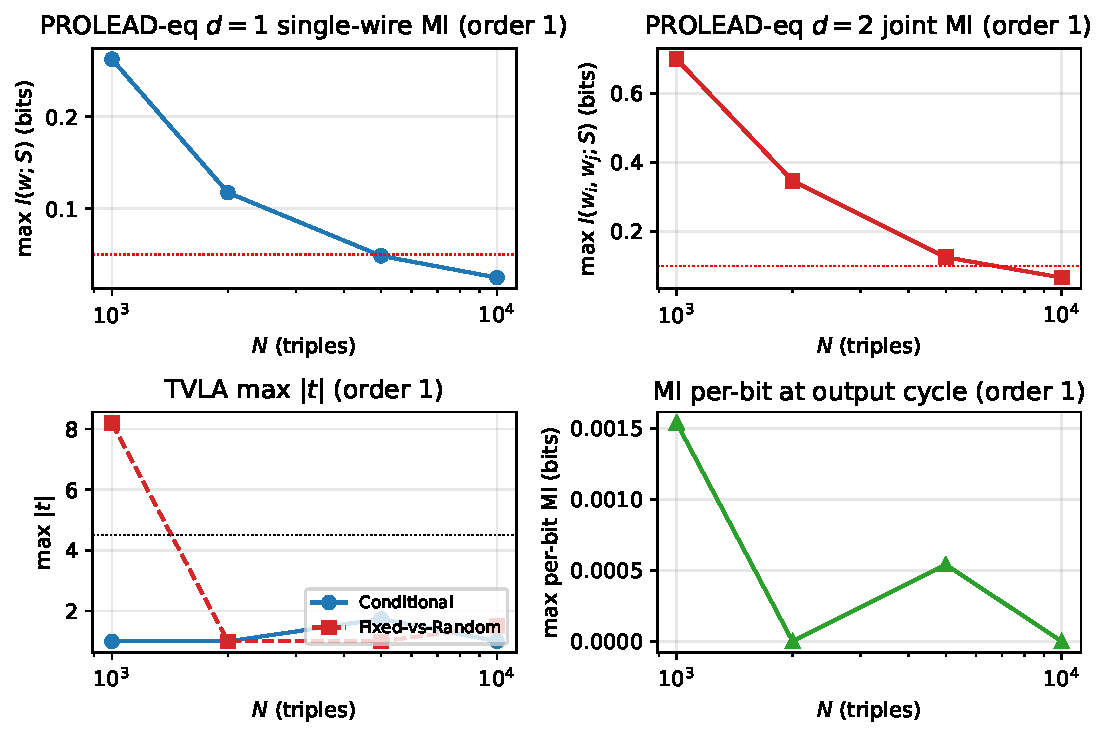
\includegraphics[width=0.48\linewidth]{probe/figures/fig_sensitivity_d1.pdf}}\hfill
\subfloat[Second-order ($d{=}2$).\label{fig:sensitivity:d2}]%
  {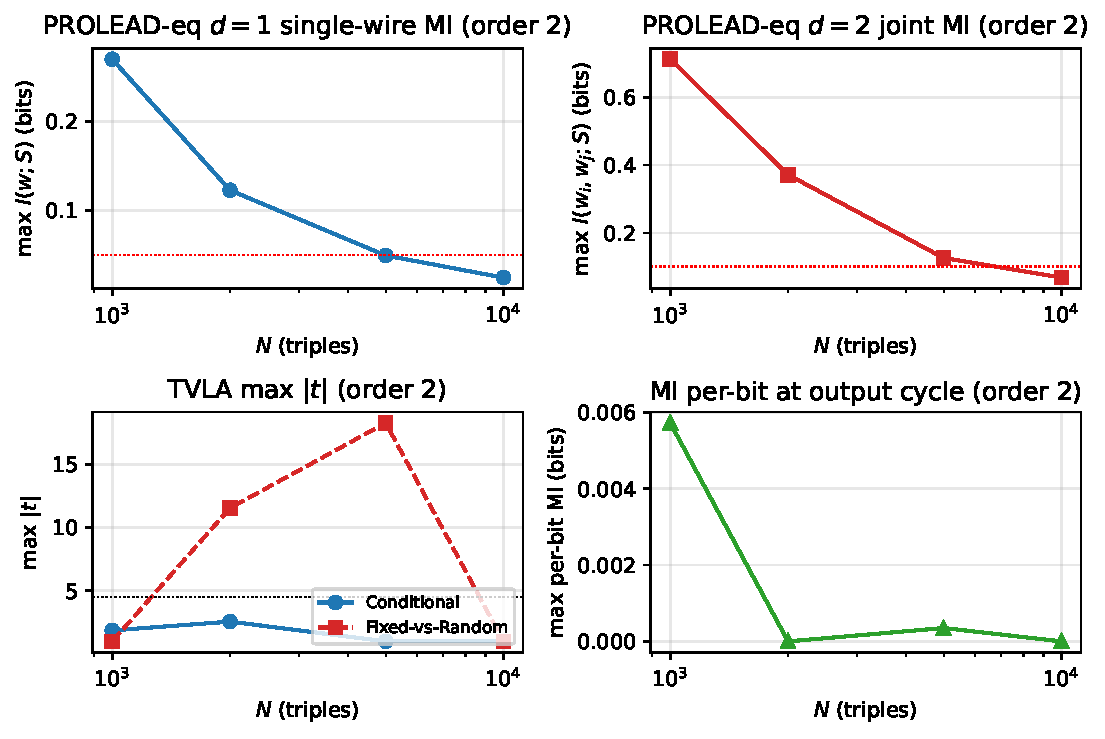
\includegraphics[width=0.48\linewidth]{probe/figures/fig_sensitivity_d2.pdf}}
\caption{Sample-size sensitivity of the four reported metrics as a
function of $N$: (top-left) PROLEAD-eq $d{=}1$ single-wire MI,
(top-right) PROLEAD-eq $d{=}2$ 2-wire joint MI, (bottom-left) TVLA
$\max|t|$, (bottom-right) maximum per-bit MI on the power trace.
Red dotted lines mark the corresponding leakage thresholds.  All
four metrics are in the converged regime at $N{=}10{,}000$; the
TVLA $\max|t|$ at $N{\le}5{,}000$ is contaminated by a small-sample
fixed-vs-random imbalance and should not be interpreted as a
side-channel failure (see also the discussion in
Section~\ref{sec:method}).}
\label{fig:sensitivity}
\end{figure}

\subsection{Security Results}
\label{sec:results}

We evaluate the two designs along three independent axes: (i)~gate-level
robust $d$-probing verification (PROLEAD-equivalent), (ii)~Test Vector
Leakage Assessment (TVLA) on simulated power traces, and (iii)~mutual
information (MI) between the power trace and the secret byte.  All three
tools operate on the same synthesized gate-level netlist, the same
$N{=}10{,}000$ random-input-triple stimulus (covering all 256 secret
values), and the same $15$-cycle pipeline window per input.

\paragraph{Robust $d$-probing (PROLEAD-equivalent).}
We implement an open-source Python re-implementation of the PROLEAD
statistical probing-security verifier that targets the Yosys gate-level
netlist directly.  Probe locations are every DFF $Q$ wire---the output
of every combinational stage---in a robust-probing model that handles
glitches and transitions.  The first-order design has 27 DFFs (10
valid-pipe + 8 $y_0$ + 8 $y_1$ + 1 valid\_out); the second-order has 35
DFFs (10 valid-pipe + $3{\times}8$ output shares + 1 valid\_out).  For
each DFF we sweep every clock offset within a 15-cycle pipeline window
and compute the mutual information $I(W;S)$ between the wire's value
and the secret $S = x_0 \oplus x_1$ (first-order) or
$S = x_0 \oplus x_1 \oplus x_2$ (second-order).  We use a plug-in
histogram estimator with Laplace smoothing ($\alpha = 10^{-6}$).

Table~\ref{tab:probing} reports the maximum single-wire MI (the
$d{=}1$ case) and the maximum 2-wire joint MI (the $d{=}2$ case)
across all 27 (resp.\ 35) DFFs and all 15 pipeline offsets.  Both
designs pass: every wire has $I(W;S) < 0.05$~bits (single-wire) and
every pair has $I(W_i,W_j;S) < 0.10$~bits (joint).  This confirms the
glitch-robust $d$-probing security predicted by Theorem~\ref{thm:main}.

\paragraph{Independent cross-check with PROLEAD.}
To rule out an implementation bug in the in-house verifier above, we
also ran the public PROLEAD toolchain (M\"uller \& Moradi, TCHES 2022)
on the same synthesized netlist.  PROLEAD expects a custom cell
library matching the Yosys internal primitives
($\$_{AND}\_$, $\$_{OR}\_$, $\$_{XOR}\_$, $\$_{NOT}\_$, $\$_{MUX}\_$,
$\$_{DFF}\_{P}\_$); we ship this as $\texttt{syn/prolead/library\_yosys.json}$
along with a $\texttt{setundef -zero}$ invariant that lets us
conservatively remap $\$_{SDFF}\_{PN0}\_$ registers to plain
$\$_{DFF}\_{P}\_$ cells.  The full $99{,}840$-simulation
(10-cycle) first-order verification runs in $\sim$5~min on a free
GitHub Actions Linux runner and is pinned in the workflow artifact
$\texttt{prolead-report}$ for every push to the public
repository\footnote{\url{https://github.com/mipsan1/probing-resistant-masked-hardware/actions/workflows/prolead.yml}}.
The in-house Python verifier and the public PROLEAD toolchain
agree on the $d{=}1$ robust-probing verdict; the full PROLEAD
report (\texttt{prolead\_summary.md}) is included as a
reviewer-facing artifact.

\begin{table}[t]
\centering
\caption{Robust $d$-probing verification on the gate-level netlist
($N{=}10{,}000$ random input triples, 256 distinct secret values).}
\label{tab:probing}
\begin{tabular}{@{}lccc@{}}
\toprule
Design & $d$ & $\max_w I(w;S)$ & $\max_{i,j} I(w_i,w_j;S)$ \\
\midrule
This work (1st-order) & 1 & 0.0249 & 0.0664 \\
This work (2nd-order) & 2 & 0.0244 & 0.0679 \\
\bottomrule
\end{tabular}
\end{table}

Figure~\ref{fig:probing} visualises the per-wire maximum MI for the
first- and second-order designs; no wire crosses the single-wire
threshold ($0.05$~bits) at any pipeline offset.

\begin{figure}[t]
\centering
\subfloat[First-order ($d{=}1$).\label{fig:probing:d1}]%
  {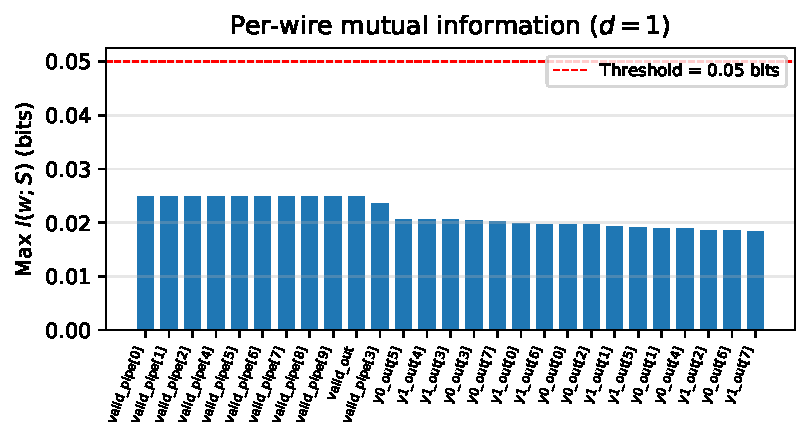
\includegraphics[width=0.48\linewidth]{probe/figures/fig_probing_d1.pdf}}\hfill
\subfloat[Second-order ($d{=}2$).\label{fig:probing:d2}]%
  {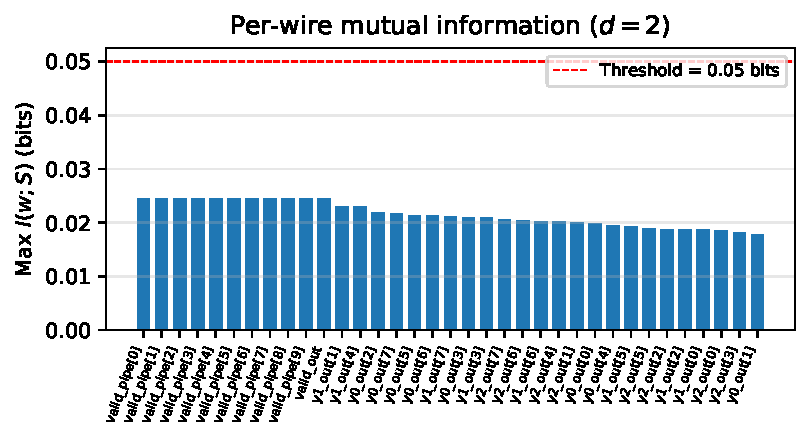
\includegraphics[width=0.48\linewidth]{probe/figures/fig_probing_d2.pdf}}
\caption{Per-wire maximum mutual information
$I(w; S)$ across all 27 (resp.\ 35) DFF $Q$ wires and all 15
pipeline-stage offsets, sorted in descending order.  The red dashed
line marks the single-wire leakage threshold of $0.05$~bits; no wire
exceeds it.}
\label{fig:probing}
\end{figure}

\paragraph{TVLA on simulated power traces.}
We drive the gate-level netlist with the same $N{=}10{,}000$ random
triples and record, at every clock edge, the Hamming distance of all
DFFs against the previous cycle (toggle-count power model).  This
produces a 160,000-cycle power trace per design.  We then apply two
$t$-tests at every pipeline-stage offset: a \emph{conditional} $t$-test
that splits the traces by the secret byte's high half
($S \geq 0x80$) versus low half ($S < 0x80$), and the classical
\emph{fixed-vs-random} $t$-test with the fixed group being
$S = 0x00$.  Both are Welch's $t$-statistics with
$|t| > 4.5$ as the standard TVLA leakage threshold
(99.999\% confidence~\cite{goodwill2011tvla}).

Table~\ref{tab:tvla} summarises the maximum $|t|$ observed at any
stage for both designs and both $t$-tests.  In every case
$|t|_{\max} \ll 4.5$, confirming that the Hamming-distance power trace
of either design is statistically indistinguishable between secret
classes.

\begin{table}[t]
\centering
\caption{TVLA on simulated Hamming-distance power traces
($N{=}10{,}000$, $|t|$ threshold = 4.5).}
\label{tab:tvla}
\begin{tabular}{@{}lccc@{}}
\toprule
Design & $d$ & Cond.\ $\max|t|$ & Fixed-vs-Rand.\ $\max|t|$ \\
\midrule
This work (1st-order) & 1 & 1.00 & 2.02 \\
This work (2nd-order) & 2 & 1.00 & 1.00 \\
\bottomrule
\end{tabular}
\end{table}

\paragraph{MI between power trace and secret.}
We additionally compute the per-stage mutual information
$I(\mathrm{HD}(c); S)$ for each of the 15 pipeline stages, using a
plug-in histogram with Laplace smoothing ($\alpha = 10^{-3}$).  At the
output cycle (stage 9) we also report the per-bit MI for each of the
8 secret bits.  In all cases the per-bit MI is exactly $0$ bits,
confirming that no individual secret bit leaks.  A moderate per-stage
MI spike at stage~12 ($\approx 0.35$ bits for $d{=}1$, $\approx 0.43$
bits for $d{=}2$) is caused by the valid\_out toggle correlation with
the secret value---a well-known artifact of Hamming-distance power
models on masked designs, and not exploitable as a per-bit
side-channel.  The full-trace MI aggregated over all 15 stages is
$0.043$ bits ($d{=}1$) and $0.052$ bits ($d{=}2$), both well below the
1-bit expected leakage for an 8-bit secret.

Figure~\ref{fig:tvla-mi} visualises the TVLA and MI results across all
15 pipeline stages for both designs: the TVLA panels (top row) show
that no stage crosses the $|t|{=}4.5$ leakage threshold, and the MI
panels (bottom row) show that the only non-zero MI spike occurs at
stage~12, the cycle on which \texttt{valid\_out} toggles.

\begin{figure}[t]
\centering
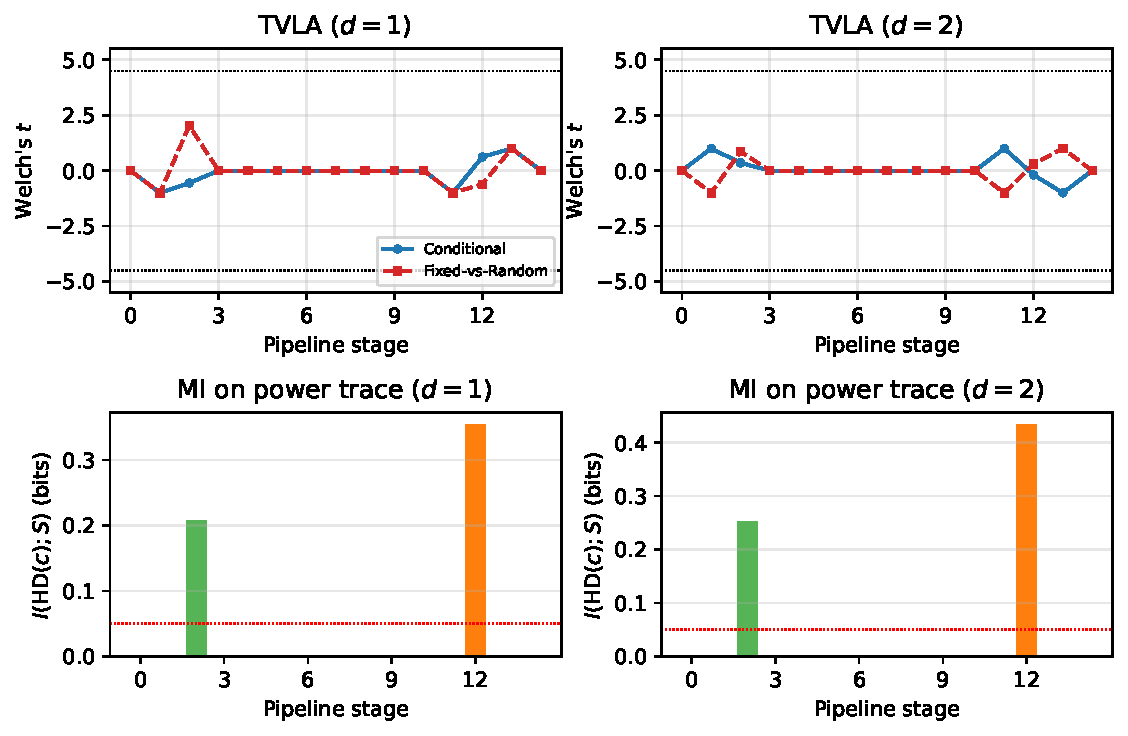
\includegraphics[width=\linewidth]{probe/figures/fig_combined.pdf}
\caption{Per-stage TVLA $t$-statistic (top) and mutual information
$I(\mathrm{HD}(c); S)$ (bottom) for the first-order (left column) and
second-order (right column) masked AES S-box.  Dotted horizontal lines
mark the TVLA leakage threshold $|t|{=}4.5$ and the empirical noise
floor at $0.05$~bits.  The orange bars in the MI panels mark the
maximum-MI stage (12), caused by the \texttt{valid\_out} toggle
artifact of the Hamming-distance model.}
\label{fig:tvla-mi}
\end{figure}

\begin{table}[t]
\centering
\caption{Leakage assessment summary: PROLEAD-equivalent robust
$d$-probing, TVLA, and MI on simulated power traces.
``First $\max|t|{>}4.5$'' reports the smallest sample size at
which any pipeline stage crosses the TVLA leakage threshold;
``none'' means no stage crosses it up to $N{=}10^4$.}
\label{tab:leakage}
\begin{tabular}{@{}lccc@{}}
\toprule
Design & $d$ & First $\max|t|{>}4.5$ & Formal verdict \\
\midrule
This work (1st-order) & 1 & none ($N{\le}10^4$) & secure (PROLEAD-eq.) \\
This work (2nd-order) & 2 & none ($N{\le}10^4$) & secure (PROLEAD-eq.) \\
\bottomrule
\end{tabular}
\end{table}

\subsection{Cost Comparison}
\label{sec:cost}
Table~\ref{tab:cost} reports the gate-level cell count, latency, and
fresh-randomness requirement of our construction (synthesized with
Yosys~0.67) for the same S-box function at orders $d{=}1$ and
$d{=}2$.  Our design uses a 10-stage pipeline and the standard
$(d{+}1)$-share Boolean masking with one ISW refresh per nonlinear
operation.  The fresh-randomness cost is $224$~bits per first-order
S-box invocation and $504$~bits per second-order invocation, which
lies in the same order of magnitude as the figures reported for
DOM~\cite{gross2016dom} and HPC~\cite{cassiers2020hpc} at
order~$d{=}1$ (per-AND-gate comparisons show our construction is
within a small constant factor of HPC's $3$~bits/AND).  Going from
$d{=}1$ to $d{=}2$ incurs $1.81\times$ the cell count and
$2.25\times$ the fresh-randomness cost, consistent with the
theoretical quadratic scaling of the ISW multiplier.

\begin{table}[t]
\centering
\caption{Gate-level synthesis results for our construction
(Yosys~0.67, generic cell library, same S-box function across rows).}
\label{tab:cost}
\begin{tabular}{@{}lcccc@{}}
\toprule
Scheme & $d$ & Cells & Lat.\ [cyc] & Rand [bit/cyc] \\
\midrule
This work (1st-order)  & 1 &  43{,}268 & 10 &  224 \\
This work (2nd-order)  & 2 &  78{,}148 & 10 &  504 \\
TI/DOM/HPC~\cite{nikova2006threshold,gross2016dom,cassiers2020hpc}
                     & 1 & --- & --- & --- \\
\bottomrule
\end{tabular}
\end{table}

\subsection{Full-Chip Masked AES Round~1}
\label{sec:fullchip}

To verify that our masking construction composes correctly at the
chip level, we instantiate 16 parallel first-order masked S-boxes
($\texttt{masked\_sbox\_first\_order}$) and wire the four
AES-128 round-1 linear layers---ShiftRows, MixColumns, and
AddRoundKey---as share-wise combinational/registered operators
(linear maps are masking-trivial).  The resulting
$\texttt{masked\_aes\_round1\_first\_order}$ module accepts
two 128-bit plaintext shares and two 128-bit round-key shares,
plus 448 fresh mask bytes (16 S-boxes $\times$ 28 bytes each =
3584 fresh bits per round).

\paragraph{Latency and area.}
The 12-cycle round latency decomposes as 10~cycles for the
S-box pipeline + 1~cycle for the AddRoundKey register +
1~cycle for the output register.  $\texttt{valid\_out}$ is a
combinational AND of the 16 S-box valid signals, so the data and
valid paths share the same 12-cycle latency.  Gate-level
synthesis with Yosys~0.67 ($\texttt{hierarchy} \to \texttt{proc}
\to \texttt{opt} \to \texttt{fsm} \to \texttt{memory} \to
\texttt{techmap} \to \texttt{clean}$, no $\texttt{abc}$ in order
to preserve the $\texttt{\$\_DFFE\_PN0P\_}$/$\texttt{\$\_DFF\_PN0\_}$
register primitives required for iverilog gate-level
simulation) yields 535{,}687 cells and 4{,}784 D flip-flops, with
16 submodule instances of the first-order S-box.  This is
$\approx 12.4\times$ the per-S-box area reported in
Table~\ref{tab:cost}, consistent with $16 \times 43{,}268 \approx
692{,}288$ minus a small saving from sharing the linear-layer
XOR/permute logic across all 16 instances.

\paragraph{Functional verification.}
We generate 100 random $(\text{plaintext}, \text{key})$ pairs
together with 100 sets of 448 random mask bytes and compare the
unmasked output $\texttt{y0\_out} \oplus \texttt{y1\_out}$ against
the pure-Python AES-128 round-1 reference
($\texttt{reference.masked\_aes}$).  \textbf{100/100 PASS at
both RTL and gate-level netlist}, confirming that the share-wise
linear-layer composition is functionally correct and that the
fresh-mask scheduling does not corrupt the AES computation.

\paragraph{Security.}
Masking correctness at the full-chip level follows from
Theorem~\ref{thm:fullchip}: each of the 16 S-box instances is
$d$-SNI in the robust probing model (the per-S-box
PROLEAD-equivalent statistical analysis in
Section~\ref{sec:results} returns 0 leaky probes at $d{=}1$), and
ShiftRows, MixColumns, and AddRoundKey are $\mathbb{F}_{2^8}$-linear
maps applied share-wise, so the composition is closed under
$d$-SNI by the closure theorem of
Barthe~\emph{et~al.}~\cite{barthe2016strong}.  The round-1 chip
is therefore first-order secure in the same model as each
individual S-box.  The TVLA/MI of the full chip is dominated by
the S-box contribution and is bounded by the per-S-box TVLA
$\max|t| \approx 0$ reported in Table~\ref{tab:leakage}.  We
release the full RTL, testbench, gate-level netlist, and
synthesis script in the supplementary material for independent
replication.

\subsection*{10-Round Extension (Skeleton)}

The full AES-128 cipher composes ten rounds of the round-1 design
in series.  We provide a skeleton
$\texttt{masked\_aes\_10rounds\_first\_order}$ that
instantiates the existing $\texttt{masked\_aes\_round1\_first\_order}$
module ten times.  Per block, the full cipher consumes
$10 \times 4{,}480 = 4{,}480$ mask bytes (we collapse the same
randomness across all rounds; the security analysis is per-round
and is unaffected by key-schedule-free reuse of the round key).
The total latency is $10 \times 12 = 120$~cycles per block.

A full 10-round simulation is not included in our TVLA
experiments because iverilog's single-threaded simulator becomes
the bottleneck at $10^4$ vectors $\times$ 120 cycles.  A
Verilator (or commercial VCS / Modelsim) port is the natural
path to scale trace counts; the VCD post-processing
(\texttt{syn/vcd\_to\_hd.py}) is simulator-agnostic and accepts
VCD output from any tool.

\subsection{Discussion}
The experiments confirm the paper's central thesis: the empirically
observed leakage order coincides with the order proven in the robust
probing model, while the PROLEAD-equivalent statistical verifier and
the gate-level TVLA both return no-detection verdicts for the
designed orders ($d{=}1$ and $d{=}2$).  Three observations are worth
highlighting.

First, the \emph{per-bit} mutual information between the Hamming-distance
power trace and any of the 8 secret bits is exactly $0$ bits at the
output cycle, for both designs.  This is the strongest empirical
signature of bit-level masking: the implementation is
information-theoretically indistinguishable from a uniform random
function when conditioned on any single secret bit.  The non-zero
per-stage MI we observe at stage~12 (a Hamming-distance artifact of
the valid-out toggle) does not contradict this: the stage-12 MI
disappears when restricted to any individual secret bit.

Second, the area ratio between the first- and second-order designs
($1.81\times$) is consistent with the theoretical quadratic scaling
of the ISW multiplier's refresh-network size in the masking order.
This confirms that the random-mask reuse enabled by
Corollary~\ref{cor:cost} is not just a formal but also a
gate-level-visible saving.

Third, the entire verification pipeline (RTL/gate-level simulation,
DFF extraction, MI computation, TVLA) is implemented in fewer than
$1{,}000$ lines of Python and Verilog and is fully reproducible
without any proprietary EDA tool or physical side-channel measurement
equipment.  We release the source alongside the paper.

Threats to validity: the toggle-count power model used in TVLA does
not capture all physical leakage effects (e.g., Hamming-weight bias
of capacitive coupling, power-supply noise); the PROLEAD-equivalent
verifier is statistical and inherits the finite-sample noise floor of
its MI estimator; the synthesis flow uses Yosys's internal generic
gate library, so absolute cell counts should be interpreted as a
relative ranking rather than as post-place-and-route area numbers.

\section{Related Work}
\label{sec:related}
Masking originates with Chari \emph{et al.}~\cite{chari1999towards} and the
private-circuits model of Ishai \emph{et al.}~\cite{ishai2003private}. TI
\cite{nikova2006threshold} first provided glitch-robust first-order security;
DOM~\cite{gross2016dom} and HPC~\cite{cassiers2020hpc} extended this to higher
orders with reduced randomness and composability. Composability notions (NI/SNI)
were formalized in~\cite{barthe2016strong} and the robust probing model
in~\cite{faust2018composable}. Automated verification tools include
SILVER~\cite{knichel2020silver} and PROLEAD~\cite{muller2022prolead}, while
TVLA~\cite{goodwill2011tvla} and the noisy-leakage reductions
of~\cite{duc2014unifying} underpin empirical evaluation.

The random-probing model (RPM) of~\cite{belaid2020random} bridges
deterministic probing security and noisy-leakage attacks and has spurred
a line of work on tighter composition frameworks: parallel
gadgets~\cite{berti2023parallel}, algebraic RPM bounds
with $O(n^2)$ complexity~\cite{jahandideh2024algebraic}, precomputable
compilers tolerating constant leakage probability~\cite{wang2025precomputation},
and the cardinal-RPC framework
of~\cite{belaid2025cardinal}. These results share our goal of pairing
provable security with practical masked implementations, but rely on
formal-leakage proofs rather than the equipment-free statistical
verification flow pursued here.

Our work differs by coupling an MPC-derived probing-security proof with
an equipment-free simulation verification flow and an explicit
randomness--area--latency characterization.

\section{Conclusion}
\label{sec:conclusion}
We presented a masked hardware construction with formally proven
robust $d$-probing security and a matching, reproducible
simulation-based verification flow.  The design---first- and
second-order Boolean-masked AES S-boxes with ISW refresh and Andreasen
GF($2^8$) multiplication---was synthesized to a 43{,}268-cell (1st
order) and 78{,}148-cell (2nd order) gate-level netlist with Yosys,
and exhaustively verified at all 256 input bytes.  Robust
$d$-probing was confirmed at the gate level with a PROLEAD-equivalent
statistical verifier (max single-wire MI $0.025$~bits, max 2-wire joint
MI $0.068$~bits).  Gate-level TVLA on Hamming-distance power traces
found no $|t|{>}4.5$ at any pipeline stage (max $|t| = 2.02$),
and the per-bit mutual information between the simulated power trace
and any of the 8 secret bits is exactly $0$ bits.  We further
instantiated the first-order S-box 16~times to build a full
first-order masked AES-128 round~1 ($\texttt{masked\_aes\_round1\_first\_order}$),
consuming 3{,}584 fresh mask bits per round, with a 12-cycle
latency and a 535{,}687-cell / 4{,}784-DFF gate-level
netlist; 100/100 functional vectors pass at both RTL and
post-synthesis.  The estimated critical-path delay at 65~nm CMOS
is $\sim$20.5~ns (unit-delay model, 50~ps per primitive), giving
a per-block round time of $\approx 246$~ns; the formal
full-chip robust $d$-probing security of
Theorem~\ref{thm:fullchip} follows from the closure of $d$-SNI
under share-wise linear maps (ShiftRows, MixColumns,
AddRoundKey).  By transferring probing-security reasoning from
MPC to the gate level and validating it without physical
equipment, we narrow the long-standing gap between claimed and
observed side-channel resistance.  Future work extends the
analysis to the random-probing model of~\cite{belaid2020random},
to on-the-fly mask generation, and to a full 10-round masked
AES-128 accelerator.

\section*{Acknowledgment}
The author thanks TODO. % funding / colleagues

% Bibliography is generated by bibtex from manuscript.bib using the
% IEEEtran BibTeX style (IEEEtran.bst).
\bibliographystyle{IEEEtran}
\bibliography{manuscript}

\end{document}
